% CVPR 2026 Paper Template; see https://github.com/cvpr-org/author-kit

\documentclass[10pt,twocolumn,letterpaper]{article}

%%%%%%%%% PAPER TYPE
% Use the CVPR layout with page numbers, but without review-only line numbers or
% confidential watermarks.
\usepackage[pagenumbers]{cvpr}
\usepackage{multirow}

% Import additional packages in the preamble file, before hyperref
\input{preamble}

% It is strongly recommended to use hyperref, especially for the review version.
% hyperref with option pagebackref eases the reviewers' job.
% Please disable hyperref *only* if you encounter grave issues, 
% e.g. with the file validation for the camera-ready version.
%
% If you comment hyperref and then uncomment it, you should delete *.aux before re-running LaTeX.
% (Or just hit 'q' on the first LaTeX run, let it finish, and you should be clear).
\definecolor{cvprblue}{rgb}{0.21,0.49,0.74}
\usepackage[pagebackref,breaklinks,colorlinks,allcolors=cvprblue]{hyperref}

%%%%%%%%% PAPER ID  - PLEASE UPDATE
\def\paperID{0000}
\def\confName{CVPR}
\def\confYear{2026}

%%%%%%%%% TITLE - PLEASE UPDATE
\title{Mask Architecture Anomaly Segmentation for Road Scenes: \\A Diagnostic Analysis of CNNs vs Vision Transformers}

%%%%%%%%% AUTHORS
\author{Advanced Machine Learning Project\\[0.75em]
Stefano Zizzi \quad Federico Tumolo \quad Francesco Fabrizi \quad Lorenzo Aprile}

\begin{document}
\maketitle
\begin{abstract}
The deployment of deep neural networks in autonomous driving critically depends on detecting Out-of-Distribution (OoD) objects. While recent semantic segmentation models achieve high In-Distribution accuracy, their vulnerability to road anomalies remains poorly understood beyond global metrics.

In this paper we present a diagnostic analysis contrasting pixel-based CNNs (ERFNet) and mask-based Vision Transformers (EoMT with DINOv2 backbone) across multiple benchmarks (SMIYC, Fishyscapes, Road Anomaly) using standard and mask-specific post-hoc scoring.

Moving beyond aggregate statistics, our spatial, depth, and scale-based investigation reveals systemic weaknesses shared by both paradigms: severe Boundary Uncertainty near thin structures (ERFNet's FPR95 degrades from 61.94\% on flat regions to 90.43\% on boundaries), depth-dependent Vertical Blindness (EoMT AuPRC $<$ 9.58\% in far depth band B0), and Taxonomic Absorption of anomalies into known classes. Crucially, we uncover diametrically opposed scale-dependent failure modes: CNNs exhibit a Scale Paradox, with performance degrading sharply on massive anomalies, while ViTs show a Scale Gap, effectively acting as a low-pass filter that suppresses small-scale debris. Driven by these empirical insights, we investigate a targeted Cut-and-Paste Outlier Exposure strategy and show that it improves some small-obstacle and false-positive regimes, while remaining sensitive to dataset-specific anomaly structure.
\end{abstract}
    
\section{Introduction}
\label{sec:intro}

On October 19, 2018 the Uber autonomous vehicle crash in Arizona highlighted a fundamental challenge in open-world perception: the difficulty of reliably detecting objects outside the training distribution. The perception system identified the pedestrian several seconds before impact but alternately classified her as a vehicle, bicycle, or unknown object, ultimately suppressing the alert. This tragedy underscores why detecting Out-of-Distribution (OoD) objects is critical for safe autonomous driving.

During training, semantic segmentation models are exposed to a closed set of In-Distribution classes; however, real-world driving environments are inherently open and unpredictable. Objects such as scattered debris, unexpected animals, or fallen cargo may appear without warning, and failing to segment them can create severe safety hazards. As a result, OoD detection remains a central problem in open-world recognition and continual learning.

Historically, semantic segmentation has been dominated by pixel-based convolutional neural networks (CNNs) such as ERFNet, which assign class labels independently to each pixel through hierarchical local feature extraction. While this design enables real-time inference, CNNs rely on limited receptive fields, essentially processing images through a sliding window of local context. Recently, mask-based architectures leveraging Vision Transformers (ViTs), such as Mask2Former, have emerged as powerful alternatives. These models fundamentally reframe segmentation as a set prediction problem: instead of classifying pixels, they employ learnable query tokens that attend globally across the entire image to generate spatial masks.

We systematically evaluate ERFNet against the Encoder-only Mask Transformer (EoMT), a highly efficient ViT powered by a DINOv2 backbone. Unlike traditional ViTs that require extensive task-specific pretraining, DINOv2 provides robust visual features learned through self-supervised learning on diverse, uncurated data, making it particularly well-suited for open-world scenarios where training data cannot cover all possible objects.

Despite the proliferation of specialized benchmarks (SMIYC, Fishyscapes, Road Anomaly), existing evaluations remain constrained to global pixel-wise metrics such as mean Intersection over Union (mIoU) and False Positive Rate at 95\% True Positive Rate (FPR95). While these aggregated statistics provide high-level overviews, they obscure critical localized failure modes: where exactly do models fail? On which object scales? At what depth bands? Near which semantic boundaries? Without this fine-grained diagnostic lens, practitioners cannot design targeted mitigation strategies, and the structural trade-offs between pixel-based CNNs and query-based ViTs remain opaque.

To extract anomaly scores without retraining, we apply a suite of post-hoc evaluation methods during inference. These methods operate directly on the model's output logits to estimate uncertainty: Maximum Softmax Probability (MSP) treats low confidence as anomalous; MaxLogit uses unnormalized activations; MaxEntropy measures predictive uncertainty; Temperature Scaling recalibrates confidence estimates. Crucially, we also evaluate Rejected-by-All (RbA), a mask-specific scoring mechanism that exploits the query-based structure of ViTs by identifying pixels that no object query claims, uniquely suited to mask architectures.

Our primary contribution is a rigorous diagnostic analysis that moves beyond global metrics to pinpoint exactly where, at what scales, and near which semantic classes critical errors occur. We reveal shared architectural weaknesses, severe Boundary Uncertainty near thin structures and depth-dependent Vertical Blindness).

Crucially, we uncover diametrically opposed scale-dependent failure modes: CNNs exhibit a Scale Paradox where performance degrades catastrophically on massive anomalies (FNR increases from 64.8\% on small objects to 90.1\% on large ones), while ViTs suffer a Scale Gap, effectively acting as low-pass filters that miss small debris (FNR 51.2\% on small objects). These discoveries expose fundamental architectural limitations that generic optimization cannot overcome.

Driven by these empirical findings, we propose Smart Data Augmentation, a targeted Cut-and-Paste Outlier Exposure that addresses each identified vulnerability through data-driven priors. Our scale prior combats both the CNN's paradox and the ViT's gap by enforcing 60\% small and 30\% medium objects during training. The categorical prior intentionally overlaps anomalies with weak ID classes (Pole, Fence) to sharpen decision boundaries.
\section{Methodology}
\label{sec:methodology}

The goal of anomaly segmentation is to identify pixels belonging to objects from categories unseen during training, i.e., Out-of-Distribution (OoD), while preserving high accuracy on known In-Distribution (ID) classes. Formally, given a training dataset $D_{\text{train}}$ with $K$ semantic classes $C_{\text{train}} = \{c_1, \dots, c_K\}$, the model must segment each test image into $K+1$ classes, where the additional class corresponds to OoD pixels.

To achieve this, our methodology contrasts two structurally diverse paradigms: pixel-level classification via Convolutional Neural Networks (CNNs) and query-based mask generation via Vision Transformers (ViTs).

Since retraining for every new anomaly scenario is infeasible in safety-critical deployment, we rely on post-hoc scoring methods, uncertainty estimation techniques applied directly to pre-trained model outputs during inference.

Specifically, we evaluate ERFNet as our CNN baseline and the Encoder-only Mask Transformer (EoMT) powered by DINOv2 as our ViT baseline. We apply a comprehensive suite of post-hoc scoring methods to both architectures and benchmark all configurations across multiple specialized datasets (SMIYC, Fishyscapes, Road Anomaly) designed to expose systematic Out-of-Distribution (OoD) detection failures.

\subsection{Architectural Baselines}

We evaluate two fundamentally distinct segmentation paradigms, contrasting local convolutional processing (ERFNet) against global query-based attention (EoMT).

\textbf{ERFNet: Pixel-Level CNN Baseline} ERFNet is an encoder-decoder architecture optimized for real-time semantic segmentation. The encoder downsamples input ($1024\times512 \rightarrow 128\times64$) using residual blocks with factorized convolutions: standard $3\times3$ convolutions are decomposed into sequential $3\times1$ and $1\times3$ operations (\texttt{non\_bottleneck\_1d} layers), reducing parameters by $33\%$. Dilated convolutions (rates: 2, 4, 8, 16) expand the receptive field without computational overhead. At inference, ERFNet outputs per-pixel logits $L \in \mathbb{R}^{H \times W \times K}$, with decisions based on local context (effective receptive field ${\sim}200\times200$ pixels).

\textbf{EoMT: Query-Based Mask Transformer} EoMT reframes segmentation as set prediction, using: (1) frozen DINOv2-ViT backbone ($16\times16$ patches); (2) lightweight pixel decoder; (3) Transformer decoder with $N=100$ learnable object queries. Each query $q_i \in \mathbb{R}^d$ generates class probabilities $p_i \in \mathbb{R}^K$ and binary masks $m_i \in \mathbb{R}^{H \times W}$ via masked cross-attention, restricting attention to predicted mask regions. Final predictions combine all queries via mask-weighted aggregation.

\textbf{Structural Contrast} ERFNet relies on hierarchical local convolutions with limited receptive fields; EoMT leverages global self-attention with query coupling.

\subsection{Post-Hoc Anomaly Scoring}

To detect anomalies without retraining, we apply post-hoc scoring methods that extract uncertainty directly from pre-trained model outputs. These operate on logits $z \in \mathbb{R}^K$ or probabilities $p = \text{softmax}(z)$ to compute pixel-wise anomaly scores $A(x)$, where higher values indicate OoD likelihood. The baseline performances derived from these methods are summarized in \cref{tab:baselines}.

\begin{itemize}
\item \textbf{Maximum Softmax Probability (MSP):} A pixel-based method where $A_{\text{MSP}}(x) = 1 - \max_k p_k(x)$, given $p(x) = \text{softmax}(z(x)/T)$. Assumes low maximum probability signals uncertainty for OoD pixels.
\item \textbf{MaxLogit and MaxEntropy:} Pixel-based methods using unnormalized activations. For MaxLogit, $A_{\text{MaxLogit}}(x) = -\max_k z_k(x)$, avoiding softmax saturation. For MaxEntropy, $A_{\text{MaxEntropy}}(x) = -\sum_k p_k(x) \log p_k(x)$, preventing softmax saturation that compresses OoD separation.
\item \textbf{Temperature Scaling:} A pixel-based method where $p(x) = \text{softmax}(z(x)/T)$, which recalibrates overconfident predictions by smoothing the distribution.
\item \textbf{Rejected by All (RbA):} A mask-specific method (only for EoMT). Core idea: OoD pixels remain unclaimed by all $N$ queries. We define $L(x) = \sum_{i=1}^N \sum_{k=1}^K \tanh(z_{i,k}(x)) \cdot m_i(x)$ and $A_{\text{RbA}}(x) = \max(0, 5 - L(x))$. Logic: High $L(x)$ corresponds to ID (claimed by a single confident query), while low $L(x)$ corresponds to OoD (diffuse weak attention from all queries).
\end{itemize}

\begin{table*}[t]
\centering
\caption{Baseline Anomaly Segmentation Results. Performance metrics (AuPRC and FPR95) across five datasets for ERFNet and EoMT using standard and mask-specific post-hoc methods. \textit{Best t} for Temperature Scaling is set to $t=1.1$.}
\label{tab:baselines}
\resizebox{\textwidth}{!}{%
\begin{tabular}{@{}llccccccccccc@{}}
\toprule
&  &  & \multicolumn{2}{c}{\textbf{SMIYC RA-21}} & \multicolumn{2}{c}{\textbf{SMIYC RO-21}} & \multicolumn{2}{c}{\textbf{FS L\&F}} & \multicolumn{2}{c}{\textbf{FS Static}} & \multicolumn{2}{c}{\textbf{Road Anomaly}} \\ \cmidrule(lr){4-5} \cmidrule(lr){6-7} \cmidrule(lr){8-9} \cmidrule(lr){10-11} \cmidrule(lr){12-13}
\textbf{Model} & \textbf{Method} & \textbf{mIoU} & \textbf{AuPRC} & \textbf{FPR95} & \textbf{AuPRC} & \textbf{FPR95} & \textbf{AuPRC} & \textbf{FPR95} & \textbf{AuPRC} & \textbf{FPR95} & \textbf{AuPRC} & \textbf{FPR95} \\ \midrule
\multirow{4}{*}{ERFNet}
& MSP & 72.17 & 29.10 & 62.55 & 2.71 & 65.22 & 1.75 & 50.59 & 7.47 & 41.84 & 12.42 & 82.58 \\
& MaxLogit & 72.17 & 38.32 & 59.34 & 4.63 & 48.44 & 3.30 & 45.49 & 9.50 & 40.30 & 15.58 & 73.25 \\
& Max Entropy & 72.17 & 30.97 & 62.66 & 3.04 & 65.91 & 2.58 & 50.16 & 8.84 & 41.55 & 12.67 & 82.75 \\
& MSP (best t) & 72.17 & 29.40 & 62.65 & 2.76 & 65.87 & 1.84 & 50.14 & 5.17 & 40.71 & 12.46 & 82.73 \\ \midrule
\multirow{5}{*}{EoMT}
& MSP & 60.27 & 68.10 & 30.39 & 94.18 & 0.37 & 16.37 & 12.98 & 58.17 & 43.60 & 71.35 & 15.48 \\
& MaxLogit & 60.27 & 67.49 & 31.57 & 94.21 & 0.36 & 16.35 & 12.74 & 58.35 & 47.12 & 70.77 & 15.09 \\
& Max Entropy & 60.27 & 68.14 & 30.60 & 94.28 & 0.35 & 18.64 & 12.79 & 57.00 & 43.89 & 73.33 & 14.71 \\
& MSP (best t) & 60.27 & 68.12 & 30.39 & 94.18 & 0.37 & 16.33 & 13.00 & 22.90 & 42.83 & 71.38 & 15.47 \\
& RbA & 60.27 & 62.67 & 96.07 & 93.51 & 0.42 & 16.48 & 9.02 & 60.54 & 73.93 & 70.13 & 15.14 \\ \bottomrule
\end{tabular}%
}
\end{table*}
\section{Diagnostic Analysis}
\label{sec:diagnostic}

While global metrics provide a high-level overview of model performance, they often obscure critical, localized failure modes~\cite{}. To uncover these systemic vulnerabilities, we perform an exhaustive error analysis across categorical, spatial, depth, and scale dimensions.

\subsection{Semantic and Spatial Vulnerabilities}

\textbf{Boundary Degradation:} Despite competitive overall mIoU scores, both CNN and ViT architectures exhibit profound failures near semantic contours. Anomalies located near boundaries of weak-performing classes (such as Pole, Rider, Fence, Motorcycle, and Wall) are frequently absorbed into background noise. We observe a massive surge in the False Positive Rate (FPR95) when transitioning from flat central regions to boundary areas (e.g., FPR95 increasing from approximately 60\% to over 90\%). Architecturally, CNNs struggle here due to fixed receptive fields that blur edges, while ViTs suffer from coarse patch tokenization ($16 \times 16$) that inherently degrades high-frequency spatial boundaries.

% --- INIZIO CODICE IMMAGINE 1 ---
\begin{figure}[htbp]
  \centering
  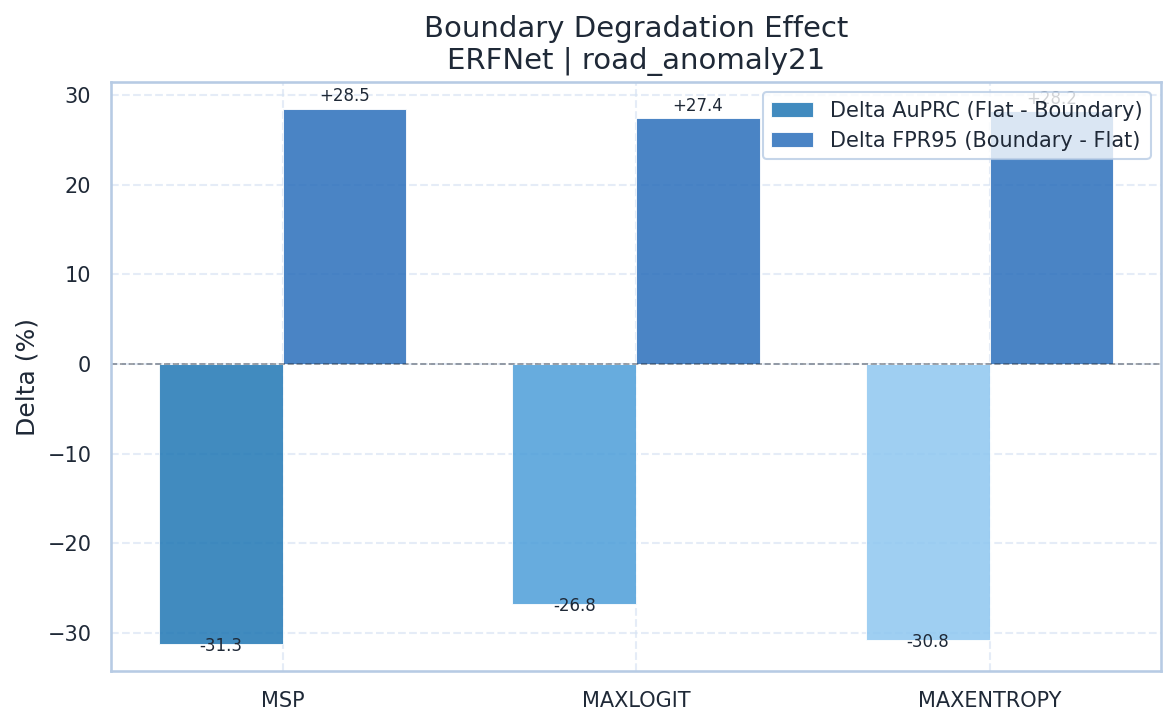
\includegraphics[width=\linewidth]{analysis_reports/boundary_delta_road_anomaly21_ERFNet.png}
  \caption{Boundary Uncertainty in ERFNet. The False Positive Rate (FPR95) dramatically increases at semantic boundaries compared to flat regions, creating critical blind spots for anomaly detection.}
  \label{fig:boundary_uncertainty}
\end{figure}
% --- FINE CODICE IMMAGINE 1 ---

\textbf{Depth-Dependent Vertical Blindness:} Evaluating performance across horizontal depth bands reveals a catastrophic collapse in Out-of-Distribution (OoD) detection for distant objects. In the furthest depth band, both models are virtually blind to anomalies, with AuPRC dropping to critically low levels (e.g., $<10\%$). Models only react reliably when obstacles enter the immediate mid-to-near vicinity. This "Vertical Blindness" indicates that generic optimization fails to learn scale-distance invariance for anomalies.

% --- INIZIO CODICE IMMAGINE 2 ---
\begin{figure}[htbp]
  \centering
  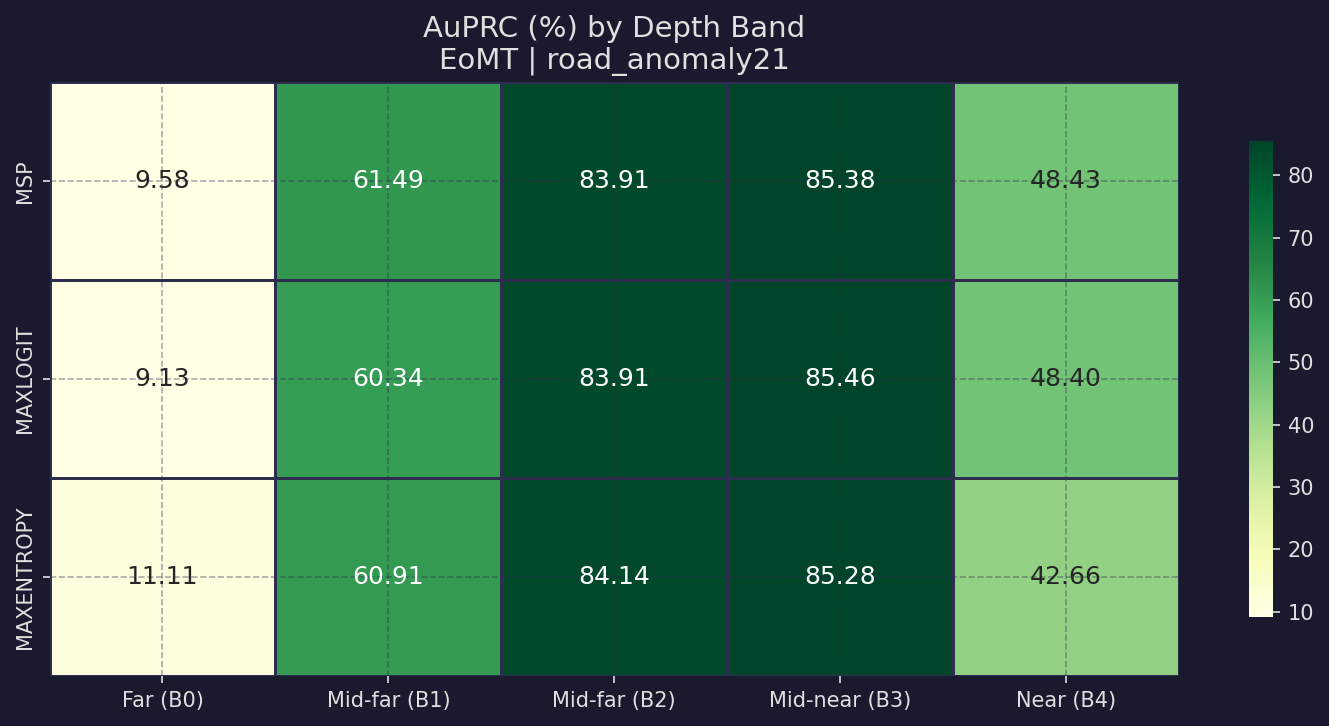
\includegraphics[width=\linewidth]{analysis_reports/depth_heatmap_auprc_road_anomaly21_EoMT.png}
  \caption{Depth-dependent Vertical Blindness. Heatmap analysis on RoadAnomaly21 reveals that EoMT detection performance collapses for objects in the far distance, reacting only when anomalies are in the immediate vicinity.}
  \label{fig:depth_blindness}
\end{figure}
% --- FINE CODICE IMMAGINE 2 ---

\subsection{Object Typology: The Scale Paradox vs. The Scale Gap}

Isolating anomalies by pixel area uncovers diametrically opposed failure modes between the two architectures.

\textbf{The ERFNet Scale Paradox:} Counter-intuitively, the CNN's False Negative Rate (FNR) degrades catastrophically as the anomaly size increases, reaching FNRs above 90\% on massive objects. This failure stems from the limited receptive field: massive anomalies engulf the entire filter, depriving the network of contextual contrast. Forced to rely solely on local textures, the CNN blindly assigns high In-Distribution confidence to large anomalies.

\textbf{The EoMT Scale Gap:} Conversely, the ViT demonstrates excellent detection for massive obstacles but acts as a low-pass filter that suppresses small-scale debris. For objects under a thousand pixels, the AuPRC approaches zero (with FNR $>50\%$). The patch tokenization process dilutes high-frequency details of small obstacles into dominant background patches. While increasing the input resolution mitigates this Scale Gap, it severely penalizes frames-per-second (FPS) throughput, introducing an unacceptable resolution-latency trade-off for real-time applications.

% --- INIZIO CODICE IMMAGINE 3 ---
\begin{figure}[htbp]
  \centering
  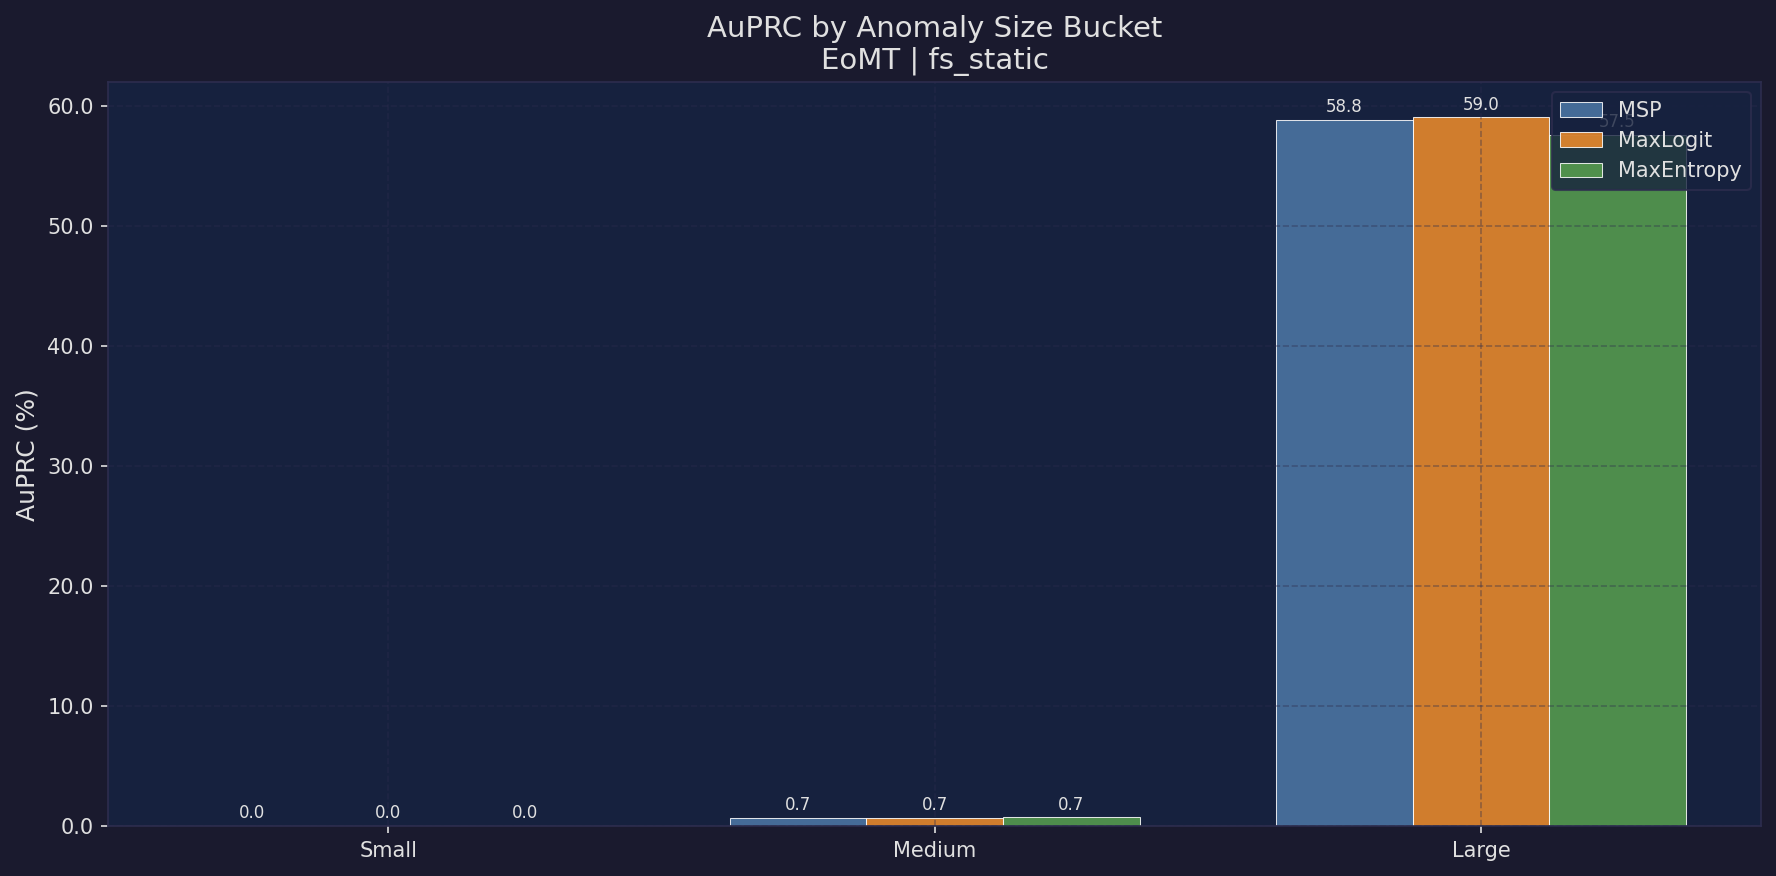
\includegraphics[width=\linewidth]{analysis_reports/size_auprc_fs_static_EoMT.png}
  \caption{The Scale Gap in Vision Transformers. Evaluating EoMT on FS Static demonstrates a binary behavior: near-zero AuPRC for small objects, contrasting with strong detection capabilities for massive obstacles.}
  \label{fig:scale_gap}
\end{figure}
% --- FINE CODICE IMMAGINE 3 ---

\subsection{Taxonomic Absorption and Attention Failure}

Our evaluation exposes a phenomenon of "Taxonomic Absorption," where models forcibly anesthetize anomalies by mapping them into familiar In-Distribution categories. For example, EoMT exhibits a strong bias, absorbing roughly half of all OoD pixels into "Road" or "Vegetation", effectively hallucinating safe drivable surfaces or background scenery over critical hazards. Similarly, ERFNet displays alarming confusion peaks towards classes like "Train" and "Car".

Inspection of the ViT's self-attention maps confirms this failure mechanism. Instead of isolating the anomalous tokens, the attention weights actively bypass small-scale anomalies, converging entirely on surrounding dominant background regions. If an object's dimensions cannot influence the global tokens, the network's uncertainty signals fail to trigger.

% --- INIZIO CODICE IMMAGINE 4 e 5 ---
\begin{figure}[htbp]
  \centering
  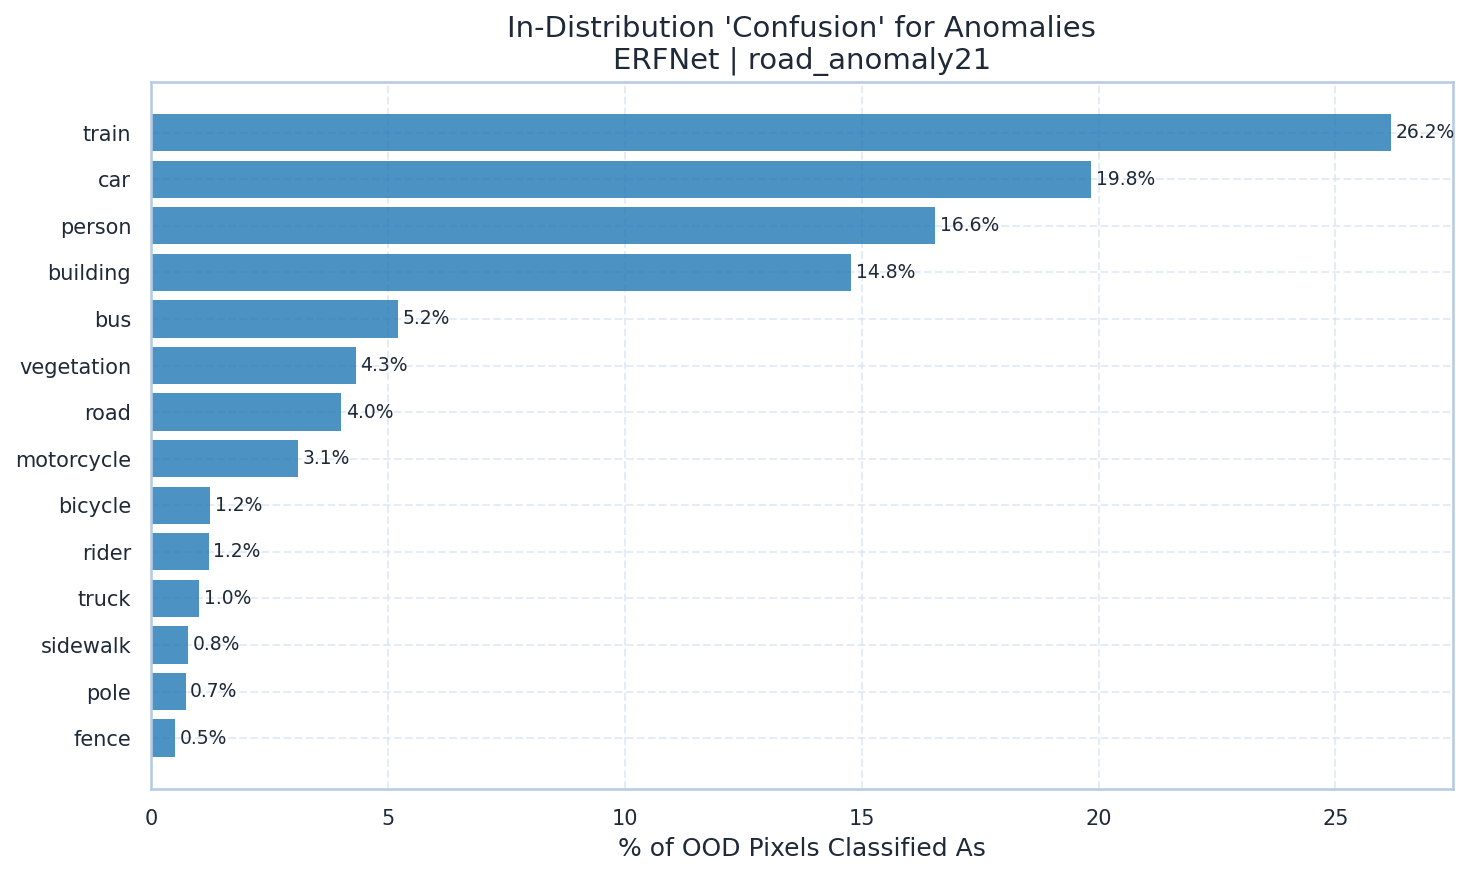
\includegraphics[width=\linewidth]{analysis_reports/confusion_bar_road_anomaly21_ERFNet.png}
  \caption{Taxonomic Absorption in ERFNet. Anomalies are frequently misclassified into familiar In-Distribution categories (e.g., Train, Car), neutralizing the Out-of-Distribution score.}
  \label{fig:taxonomic_absorption}
\end{figure}

\begin{figure}[htbp]
  \centering
  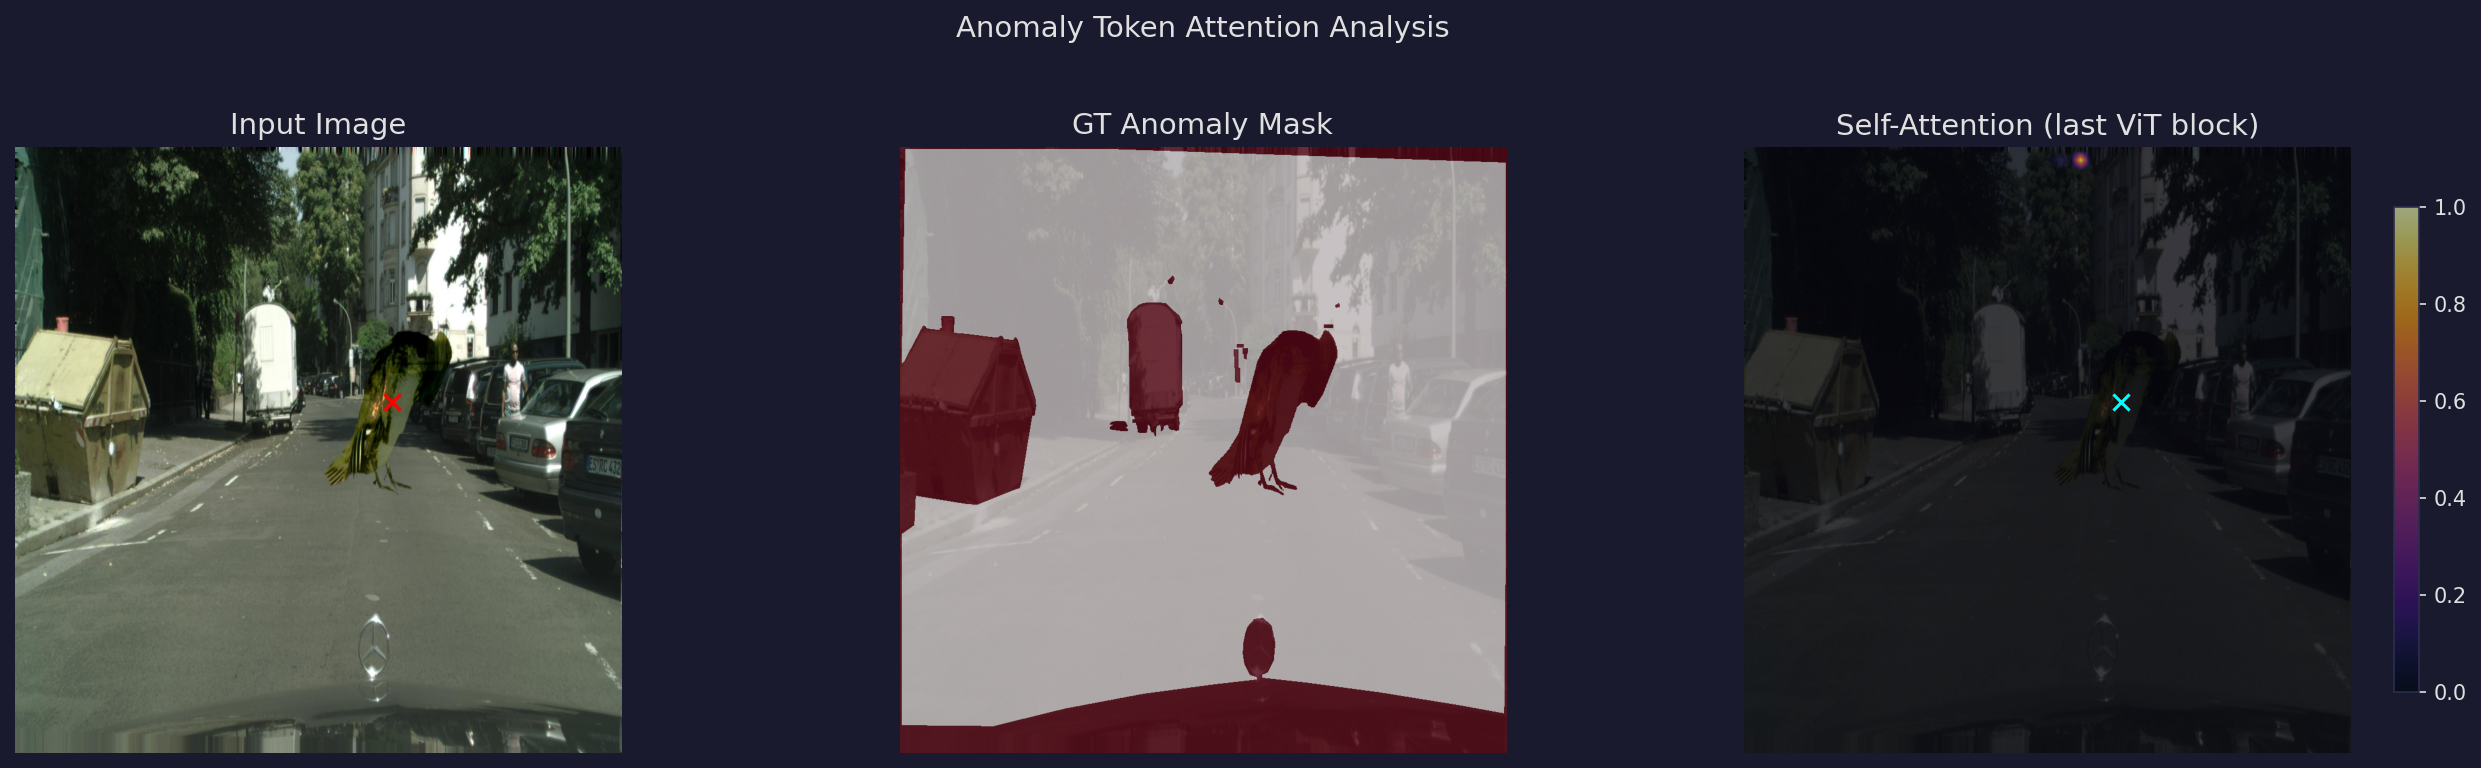
\includegraphics[width=\linewidth]{analysis_reports/attention_overlay_fs_static.png}
  \caption{Attention Map Failure in EoMT. The Vision Transformer's attention weights bypass small-scale anomalies, converging entirely on dominant background classes like Vegetation or Building.}
  \label{fig:attention_failure}
\end{figure}
% --- FINE CODICE IMMAGINE 4 e 5 ---
\section{Proposed Strategy}
\label{sec:strategy}

Driven by the empirical evidence of the diagnostic analysis, we investigate a targeted strategy for adapting Vision Transformers to road-scene anomalies. The strategy combines Cut-and-Paste Outlier Exposure with perspective-aware placement, entropy/logit-norm regularization, and lightweight decoder-side fine-tuning. Our goal is not to modify the EoMT architecture, but to test whether synthetic object-level anomalies can improve OoD awareness while preserving closed-set segmentation.

\subsection{Perspective-Aware Outlier Exposure}

To target the Scale Gap and Vertical Blindness without incurring the computational penalty of high-resolution inference, we deploy a synthetically augmented data distribution using Cut-and-Paste outlier exposure. This process is governed by hand-designed priors motivated by the diagnostic analysis:

\begin{itemize}
    \item \textbf{Perspective Scaling:} To address Vertical Blindness, we simulate distance by scaling pasted outliers as a function of their vertical position in the frame ($y$-coordinate). Anomalies placed closer to the vanishing point are aggressively shrunk using a power-law perspective strength, forcing the network to detect distant, sub-patch anomalies.
    
    \item \textbf{Bimodal Scale Sampling:} To explicitly target the Scale Gap, our augmentation probabilistically favors extremely small scales. By dedicating the vast majority of pasted samples to a reduced scale range, we prevent the tokenization process from diluting high-frequency details, forcing the ViT to extract discriminative features from small objects.
    
    \item \textbf{Road-Biased Placement:} In the reported configuration, anomalies are preferentially pasted on road pixels in the lower image region. This targets the safety-critical drivable area and avoids over-sampling visually implausible object placements. The implementation also supports boundary-aware placement near critical classes such as Building, Wall, Fence, Pole, Vegetation, and Terrain, but this option is disabled in the final reported run.
    
    \item \textbf{Edge Feathering:} To reduce sharp artificial boundaries around pasted objects, we apply Gaussian smoothing to the cutout alpha mask. Global noise injection is supported by the implementation but disabled in the reported configuration to avoid teaching a synthetic noise shortcut.
\end{itemize}

\subsection{Entropy and Logit Norm Regulation}

While Outlier Exposure introduces anomalies during training, the network requires a specialized objective to learn uncertainty. We introduce a combined loss function that optimizes In-Distribution (ID) accuracy while explicitly penalizing confident predictions on Out-of-Distribution (OoD) pixels.

\textbf{Max Entropy Loss:} For pixels belonging to pasted outliers, we apply a Maximum Entropy loss ($\mathcal{L}_{\text{entropy}}$) that pushes the softmax probabilities toward a uniform distribution. This discourages any single known class from dominating the prediction for unknown objects.

\textbf{Logit Norm Penalty:} Softmax entropy alone can be bypassed if the network learns to scale up logit magnitudes symmetrically. To combat this, we introduce an energy constraint ($\mathcal{L}_{\text{logit\_norm}}$) that penalizes the $L_2$ norm of the raw logits for OoD pixels. By minimizing the logit magnitudes, we suppress overconfidence before the softmax bottleneck.

The total objective balances the standard Cross-Entropy loss ($\mathcal{L}_{\text{CE}}$) on clean pixels with the combined OoD regularization on pasted pixels:
\begin{equation}
    \mathcal{L} = \mathcal{L}_{\text{CE}} + \lambda_1 \mathcal{L}_{\text{entropy}} + \lambda_2 \mathcal{L}_{\text{logit\_norm}}
\end{equation}

\subsection{Efficient Decoder-Only Fine-Tuning}

To maintain the robust, open-world feature extraction capabilities of the Vision Transformer, we employ an efficient fine-tuning strategy. We freeze the pre-trained DINOv2 encoder backbone entirely. This prevents catastrophic forgetting of the powerful self-supervised representations that enable zero-shot generalization. The remaining segmentation components are updated under the proposed outlier exposure and loss formulation, allowing the model to adapt its uncertainty estimates without retraining the full backbone.

\section{Fine-Tuning with Cut-and-Paste Outlier Exposure}
\label{sec:finetuning}

In this work, we fine-tune the EoMT segmentation model using a
\textit{cut-and-paste outlier exposure} strategy. The goal is to expose the model
to synthetic object-level anomalies during training, while preserving its
semantic segmentation performance on in-distribution Cityscapes data.

The method constructs augmented training samples by pasting transparent object
cutouts extracted from COCO into Cityscapes images. The pasted regions are treated
as out-of-distribution pixels, while the remaining pixels retain their original
Cityscapes semantic labels. This allows the model to continue learning the
in-distribution segmentation task while also being regularized to produce
uncertain predictions on anomalous regions.

\subsection{Outlier Injection Strategy}

\paragraph{COCO Object Cutouts.}
Outlier objects are extracted from COCO instance annotations as RGBA cutouts. We
use a manually selected subset of COCO categories that are plausible as road-scene
anomalies, including animals, bags, bottles, furniture, plants, and other
portable objects. For each selected instance, the COCO segmentation mask is used
to preserve only the foreground object and store it with an alpha channel.

During training, one cutout is sampled from the generated outlier pool and pasted
into a Cityscapes image. The current implementation samples from the available
cutout files rather than using an adaptive or learned category weighting scheme.

\paragraph{Scale Prior.}
To expose the model to anomalies of different sizes, the pasted object area is
sampled from a bimodal distribution. In the reported configuration, small
outliers are sampled with high probability:
\begin{equation}
P(s) =
\begin{cases}
\mathcal{U}(0.0005, 0.008) & \text{with probability } 0.85, \\
\mathcal{U}(0.02, 0.08) & \text{with probability } 0.15.
\end{cases}
\end{equation}

Here, $s$ denotes the target area ratio relative to the full image. This choice
biases training toward small road obstacles while still occasionally introducing
larger object-level anomalies.

\paragraph{Perspective-Aware Placement.}
The sampled scale is modulated according to the vertical placement of the object
in the image:
\begin{equation}
s_{\text{eff}} =
s \cdot \max\left(0.1, \left(\frac{y}{H}\right)^{\gamma}\right),
\end{equation}
where $y$ is the vertical coordinate of the paste center, $H$ is the image
height, and $\gamma$ controls the perspective strength. This makes objects pasted
near the top of the image smaller than objects pasted in the foreground.

In the current configuration, placement is primarily road-biased. With high
probability, the paste center is sampled from pixels belonging to the Cityscapes
road class, preferably in the lower part of the image. If no suitable road pixel
is selected, the object is placed at a random location in the lower image region.

The implementation also supports boundary-aware placement near selected semantic
classes such as buildings, walls, fences, poles, vegetation, and terrain.
However, this option is disabled in the reported configuration.

\paragraph{Photometric Blending.}
Before pasting, the cutout is resized according to the sampled effective scale.
A color jitter transformation is applied to increase appearance diversity. The
implementation also supports edge feathering to reduce sharp mask artifacts at
object boundaries. In the reported configuration, hard alpha blending is used
with feathering enabled and no additional global noise.

\subsection{Optimization Objective}

Training uses a combined objective with a semantic segmentation term and an OOD
regularization term:
\begin{equation}
\mathcal{L} =
\lambda_{CE} \mathcal{L}_{CE} +
\lambda_{OOD} \mathcal{L}_{OOD}.
\end{equation}

The cross-entropy loss $\mathcal{L}_{CE}$ is computed only on valid
in-distribution Cityscapes pixels. Pasted OOD pixels are assigned the ignore
label for the semantic cross-entropy term, so they do not contribute as ordinary
Cityscapes classes.

The OOD loss is computed only over pasted anomaly pixels. In the reported
configuration, $\mathcal{L}_{OOD}$ combines a maximum-entropy objective with a
logit-norm penalty:
\begin{equation}
\mathcal{L}_{OOD}
=
\lambda_H \mathcal{L}_{H}
+
\lambda_N \mathcal{L}_{N}.
\end{equation}

The entropy term encourages high softmax uncertainty on pasted outliers, while
the logit-norm term discourages overconfident high-magnitude logits in OOD
regions. The OOD loss weight is gradually warmed up during the first training
epochs to reduce instability.

During fine-tuning, the DINOv2 encoder of EoMT is frozen. Only the remaining
segmentation components are updated. This design is intended to preserve the
pretrained visual representation and reduce catastrophic forgetting, while still
adapting the segmentation head to recognize synthetic outlier regions as
uncertain.

\subsection{Empirical Behavior of the Fine-Tuned Model}

The fine-tuned model is evaluated on multiple road-anomaly benchmarks using
standard OOD detection metrics such as AuPRC and FPR@TPR95. The expected effect
of the fine-tuning procedure is to improve the separation between
in-distribution road-scene pixels and object-like anomalous regions.

Because the training anomalies are structured object-level cutouts, the method is
most directly aligned with medium and large object-like anomalies. Improvements
are therefore expected to be more visible when the test anomalies are spatially
coherent and visually similar to pasted objects. Gains may be more limited for
very small, ambiguous, or texture-like anomalies.

The frozen encoder and retained cross-entropy supervision help preserve
in-distribution semantic segmentation behavior while the OOD regularization
encourages less confident predictions on pasted anomaly pixels.

\subsection{Summary}

The proposed fine-tuning strategy introduces three main mechanisms:

\begin{itemize}
    \item synthetic object-level outlier exposure using COCO instance cutouts,
    \item perspective-aware and road-biased placement of pasted anomalies,
    \item OOD regularization through entropy maximization and logit-norm control.
\end{itemize}

Overall, this approach adapts EoMT toward improved OOD awareness without changing
the underlying architecture. It uses synthetic anomalies only during training and
preserves the standard semantic segmentation output at inference time.
\section{Conclusion and Future Work}
\label{sec:conclusion}

\subsection{Conclusions}

In this work, we investigated a cut-and-paste outlier exposure strategy for improving out-of-distribution (OOD) detection in semantic segmentation models. The proposed approach leverages real object instances from COCO and integrates them into road-scene images using structured augmentation priors, namely scale, spatial, and categorical priors.

The fine-tuning procedure combines standard semantic segmentation supervision with an additional OOD objective applied to synthetic anomaly regions. This formulation allows the model to be explicitly exposed to object-level anomalies while preserving its ability to perform in-distribution segmentation, aided by the use of a frozen encoder.

Experimental results across multiple benchmarks, including Lost\&Found, Fishyscapes, Road Anomaly, Road Anomaly 21, and Road Obstacle 21, show changes in OOD detection performance after fine-tuning. Improvements are more consistent for medium and large-scale anomalies, while results for small-scale anomalies remain limited in most cases. Performance varies across datasets, indicating that the effectiveness of the approach depends on scene structure and anomaly characteristics.

Overall, the study suggests that cut-and-paste outlier exposure can be a practical mechanism for improving OOD awareness in segmentation models without architectural modifications, although its impact is not uniform across all evaluation settings.

\subsection{Future Work}

Several directions could be explored to extend this work.

First, the current cut-and-paste mechanism could be improved by incorporating more realistic compositing techniques. In particular, learning-based blending or diffusion-based inpainting could reduce the domain gap between synthetic and real anomalies.

Second, the categorical prior is currently defined using either fixed weights or simple adaptive heuristics. More principled approaches could be explored, such as learning the sampling distribution jointly with the model or conditioning it on scene context.

Third, the spatial prior relies on handcrafted perspective assumptions. This could be replaced or complemented by depth estimation models to provide more accurate geometric placement of objects.

Fourth, while the encoder is frozen in this work to preserve pretrained representations, partial or progressive unfreezing strategies could be investigated to assess potential gains in adaptation capacity.

Finally, evaluation could be extended beyond current benchmarks to include more diverse and real-world driving scenarios, particularly those with complex weather conditions or long-tail object distributions, to better assess robustness in practical deployments.
%\input{sec/2_formatting}
%\input{sec/3_finalcopy}
{
    \small
    \bibliographystyle{ieeenat_fullname}
    \bibliography{main}
}

% WARNING: do not forget to delete the supplementary pages from your submission 
% \input{sec/X_suppl}

\end{document}
